\chapter*{Acknowledgments}

I have a secret hobby of reading other people's acknowledgments section in their dissertations. I can't believe I'm now writing my own. Well, it's gotten to this part of the Ph.D. Lots of mixed emotions about the last few years, mostly positive ones, but we're here to thank people, so here we go:

\setlength{\intextsep}{0em}
\begin{wrapfigure}{r}{0.3\linewidth}
  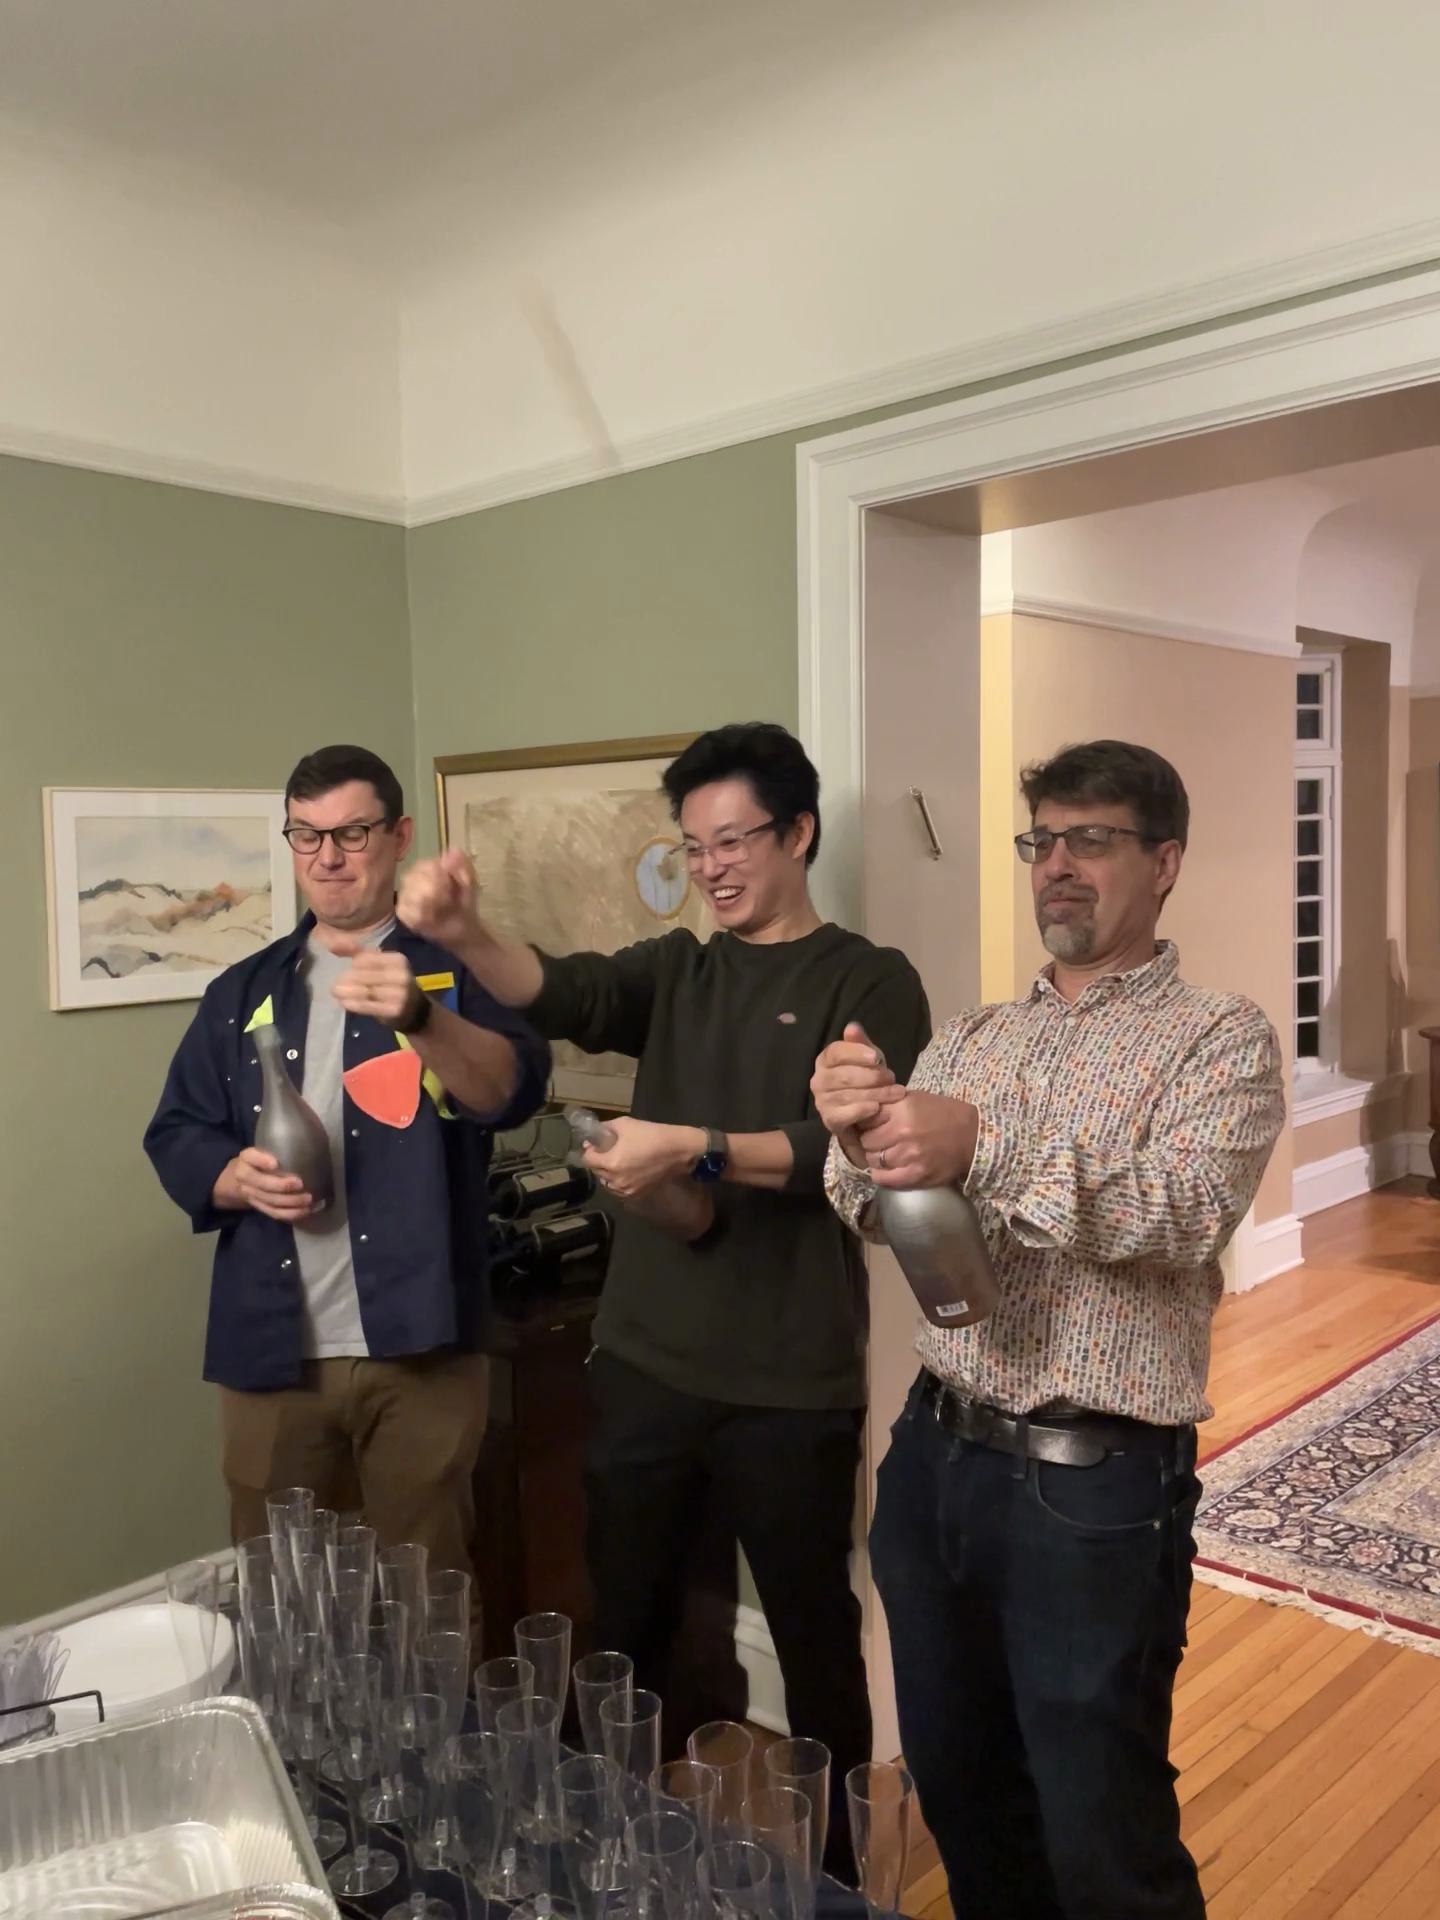
\includegraphics[width=\linewidth]{assets/josh-and-ken.png}
  \vspace{-.5\baselineskip}\caption{The author of this dissertation (\figloc{middle}) and his doctoral co-advisors, Josh (\figloc{left}) and Ken (\figloc{right}), opening bottles of champagne some day after the defense.\label{fig:josh-and-ken}}
\end{wrapfigure}
First, thank you to my co-advisors \textbf{Josh Sunshine} and \textbf{Ken Koedinger}. Josh brought me into Carnegie Mellon University (CMU) in 2017 as a Research Experiences for Undergraduates in Software Engineering (REUSE) student. In the summer of REUSE, I built out an early version of \Penrose and had the best time ever. That summer I learned that building software can be cool, and it drove me to do this Ph.D. Crucially, Josh kept me moving forward, not just in that summer, but also during my Ph.D. In 2018, I joined CMU as a Ph.D. student, and needed to find a co-advisor. I cold-emailed Ken in my first week about my interests in diagramming and his prior work on diagram configurations and chunking~\cite{koedinger_emergent_1992}. 16 days later, I got an email from Ken (\textit{``That's an amazingly slow reply!!''} said Josh). A meeting later, we started working together. Frankly, both Josh and I were complete amateurs in Ken's research areas, and we simply bonded with Ken over the same intellectual curiosities about visual representations and how to help people learn better with diagrams. Ken was extremely patient in guiding me as I struggled to come up with good research projects in the first few years. When I was in need of resources, Ken would never hesitate to help. I'm truly grateful to have Ken as my advisor. 

My undergraduate advisors, \textbf{John MacCormick} at Dickinson College and \textbf{Stephen Edwards} at Columbia University got me into research and I will always be grateful for their guidance in my formative years as a researcher. I'd also like to thank members of my thesis committee for providing valuable feedback since my thesis proposal: \textbf{Brad Myers}, \textbf{Shriram Krishnamurthi}, and \textbf{Titus Barik}. In addition my official advisors, some senior researchers mentored me and helped me grow as a researcher: \textbf{Keenan Crane}, \textbf{Jonathan Aldrich}, \textbf{Michael Hilton}, \textbf{Chinmay Kulkarni}, \textbf{Ravi Chugh}, and \textbf{Sarah Chasins}.

\Penrose wouldn't exist without the great people who worked passionately and tirelessly together on it. For that, I owe a lot to the \Penrose team and the open-source community. Josh, Keenan, Jonathan, and \textbf{Kai Ye} had been my mentors and colleagues on \Penrose since day one. This founding team of people came from very different research areas, but shared the same goal of making a good diagramming tool. This goal is not merely a ``research vision,'' but a concrete desire to build something better and to ship it for real. It's unusual in the research world to have this desire, and it brought many challenges over the years. Are we building the right thing? Should we write $X$ in the system? Do we publish? If so, where? How often? Do we keep building or do we evaluate? I still don't have answers to many of these questions. It's just difficult to do interdisciplinary research while trying to build an actual open-source system. Yet despite the difficulties, the team kept going and built \Penrose, which I am very proud of. Over the years, many great students and researchers joined the ``core team'' and contributed significantly to \Penrose. I learned tremendously from each of them and would like list some things I learned: Kai is my first Ph.D. mentor, who taught me how to lead a diverse team like \Penrose and communicate my work both within the team and to the world. I have a ton of respect for Keenan, who elevated the standard of scientific communication for the entire team and showed us the frontier of expert-quality diagramming. Jonathan introduced me to programming language design, a central topic for \Penrose till this day. \textbf{Sam Estep} single-handedly improved \Penrose's performance by $100\times$ and taught me how to build elegant and performant software. Without \textbf{Max Krieger}, I won't know how to build any web applications nor how to build anything cool and fun. 
\textbf{Yiliang ``Leo'' Liang} has built many of the language features in \Penrose and spent many hours teasing out obscure corner cases for every single feature. \textbf{Ji\v{r}\'{i} Minar\v{c}\'{i}k} is the first core contributor from the open-source community, and I always learn from his beautiful demos that push the limits of \Penrose. \textbf{Hwei-Shin Harriman} built \Edgeworth from scratch during her summer internship, and we've bonded over many things research and non-research. In my last summer at CMU, I was fortunate to have both \textbf{Kyle Lee} and \textbf{Griffin Teller} on the \Penrose team, both of them are turbo-charged CMU undergrads who showed me a level of intellectual curiosity and work ethics that I'd never achieve as an undergrad. There are many other students who worked on \Penrose as core team members, and I'm fortunate to have worked with you all: \textbf{Rijul Jain}, \textbf{Raven Rothkopf}, \textbf{Matt Davis}, \textbf{Rain Du}, \textbf{Josh Pollock}, \textbf{Lily Shellhammer}, \textbf{Mia Tang}, \textbf{Stella Trout}, \textbf{Jenna Wise}, and \textbf{Helena Yang}. Among the contributors to \Penrose, I'd like to thank \textbf{Wojtek Nawrocki} for integrating \Penrose into Lean's \texttt{ProofWidgets4} and \textbf{Steven Clontz} for introducing \Penrose and myself to the great \texttt{code4math} community. Our open-source development also received support from CMU: thank you \textbf{Tom Hughes} and \textbf{Sayeed Choudhury} for your advice and supporting me via the ``CMU Open Source Office Fellowship, supported by the Alfred P. Sloan Foundation,'' the only fellowship I'd ever get because nobody gives me fellowships for whatever reason, no matter how long my essays are. 

I play pool, and this sport\footnote{I'll play a race to 7 of 10-ball with anyone who doesn't think it's a sport.} kept me sane throughout my Ph.D. I treat pool as my second career and aim to be a third-rate professional player at some point. I didn't achieve that during the Ph.D. but I am working hard towards this goal. 33\% of my grad school choice came down to the availability of pool tables, and CMU turned out to be the best possible place to be. I'm fortunate to become friends with and opponents of many great pool players over the years: \textbf{Zixin Wen}, \textbf{Brian Zhang}, \textbf{Yifu Cai}, \textbf{Andrew Spoto}, \textbf{Linpeng ``Larry'' Chen}, \textbf{Matthew Dai}, \textbf{Zixu ``Elias'' Lu}, \textbf{Ziniu ``Eric'' Wu}, \textbf{Ruoyuan ``Ryan'' Liu}, \textbf{Shitong ``Michael'' Pang}, \textbf{Andrew Fu}, \textbf{Shanshan Xie}, \textbf{Koutian Huang}, \textbf{Jiapeng ``Billy'' Zhou}, \textbf{Ava Schieferstein}, \textbf{Wayne Lam}, \textbf{Junyu Huang}, \textbf{Peter Hammer}, \textbf{Ian Morales}, \textbf{Titus Priscu}, \textbf{Josh Phillips}, \textbf{Elina Lee}, \textbf{Zelin Ye}, \textbf{Dean Jongwattanasinkul}, \textbf{Ryan Lin}, \textbf{Eric Wang}, \textbf{Hossein Baktash}, \textbf{Yuxiao ``Nick'' Chen}, \textbf{Spencer Allen}, \textbf{Animesh Ghose}, \textbf{Pan Wang}, \textbf{Zhongwei ``William'' Ren}, \textbf{Richard Wang}, \textbf{Sida Cheng}, \textbf{Eddie Martinez}, \textbf{Matt Shen}, \textbf{Mai Zhang}, \textbf{Yushi Hou}, \textbf{Chuck Farinella}, and \textbf{Mike Shamos}. Not everything in life is about work, and I have no lessons learned from pool that can help my research directly. However, the long practice hours and careful studying of the game did teach me to appreciate anyone who takes their thing seriously, no matter what the thing is. So I appreciate everyone who does not give up their thing for a job, has ambitions in their hobbies, and spends the hours to perfect their thing. Pool commentators like to say ``pool gods'' to refer to the randomness in the game. I don't believe in them, but believe in hard work and deliberate practice. Therefore, the dedication to pool gods a few pages before was a joke. Obviously this document is dedicated to my family, but I just wanted open with something in my character.

Having passed the age to actively make friends, I'm extremely fortunate to become friends with many at CMU: \textbf{Zeeshan Lakhani}, \textbf{Daye Nam}, and \textbf{Christopher Meiklejohn} are my peers in the Ph.D. program. Both Zeeshan and Chris had much more challenging circumstances in the Ph.D. than I did, \eg Zeeshan juggled a full-time job, a very lovely family, and the actual Ph.D. research. Despite all that, both of them showed me what is good work and how to dedicate oneself to do good work. From Zeeshan in particular, I learned tremendously about research and life from our many conversations over coffees and drinks, in bars and around campus. Daye and I shared the same offices throughout the Ph.D. and we enjoyed matching Korean and Chinese words together. I'm sure both of us will always remember the first long conversation we had during Ph.D. visit days, and many others in our office. Speaking of the offices, my officemates in both Wean 5309 and TCS 317 are my closet support group and friends for life: Daye, \textbf{Morgan Evans}, \textbf{Ryan Zheyuan Shi}, \textbf{Melrose Roderick}, \textbf{Jane Hsieh}, and \textbf{Matthew Shneider}. Despite how difficult it was to park around CMU, I always enjoyed going to the office because of them and many other friends at CMU. I enjoyed conversations with many of you in the hallways, around the espresso machine, and other random places: \textbf{Simon Chu}, \textbf{Ao Li}, \textbf{Daniel Ngo}, \textbf{Jenny Liang}, \textbf{Manisha Mukherjee}, \textbf{Kyle Liang}, \textbf{Peter Carragher}, \textbf{Jenna Wise}, \textbf{Chu-Pan Wong}, \textbf{Shurui Zhou}, \textbf{Tom Magelinski}, \textbf{Ivan Ruchkin}, \textbf{Ashutosh Pandey}, \textbf{Yining She}, \textbf{Haoze He}, \textbf{Sophia Kolak}, \textbf{Courtney Miller}, \textbf{Vasu Vikram}, \textbf{Changjian ``CJ'' Zhang}, \textbf{Aidan Yang}, \textbf{Elizabeth Gilbert}, \textbf{Luke Dramko}, \textbf{Nadia Nahar}, \textbf{Hongbo Fang}, and \textbf{Aidan Yang}. In addition to human friends, there are a few great fluffy friends I appreciate around TCS: \textbf{Chanel}, \textbf{Mei}, \textbf{Tater}, \textbf{Moonie}, \textbf{Flynn}, and \textbf{Truffle}. 

Outside of the S3D program, I was lucky to have met many good Ph.D. friends: \textbf{Michael Xieyang Liu} and I are one year apart in the Ph.D. but shared many struggles and happy memories during the program, and we even became neighbors for a while. \textbf{Rohan Sawhney} gave me a lot of great advice throughout my Ph.D. and was always there whenever I had difficult career decisions to make. Folks in the HCI+PL community such as Josh Pollock, \textbf{Will Crichton}, \textbf{David Moon}, \textbf{Brian Hempel}, and \textbf{Justin Lubin} always gave me many inspirations in our conversations at various conferences and workshops. I had a great time during my 2022 internship in Seattle and met some great friends that I stayed in touch with: \textbf{Rebecca Krosnick}, \textbf{Gabriel Matute}, \textbf{Samantha Robertson}, and \textbf{Nava Haghighi}. Peers I met in other contexts and want to thank include: \textbf{Xu Wang}, \textbf{Xiaofei Zhou}, \textbf{Wesley Hanwen Deng}, \textbf{Amber Horvath}, \textbf{Jianzhe Gu}, \textbf{Nick Sharp}, \textbf{Jingya Chen}, \textbf{Sam Lau}, \textbf{Yixin Wu}, \textbf{Jingxi Xu}, and many others. Similarly, some fluffy friends outside of TCS: \textbf{Draky}, \textbf{Louie ``Popcorn'' Ogawa}, \textbf{Cece}, \textbf{Mars Wang}, \textbf{Scampi}, \textbf{Hex}, \textbf{Octo}, and \textbf{Ruby}.

\begin{figure}[t]
    \centering
    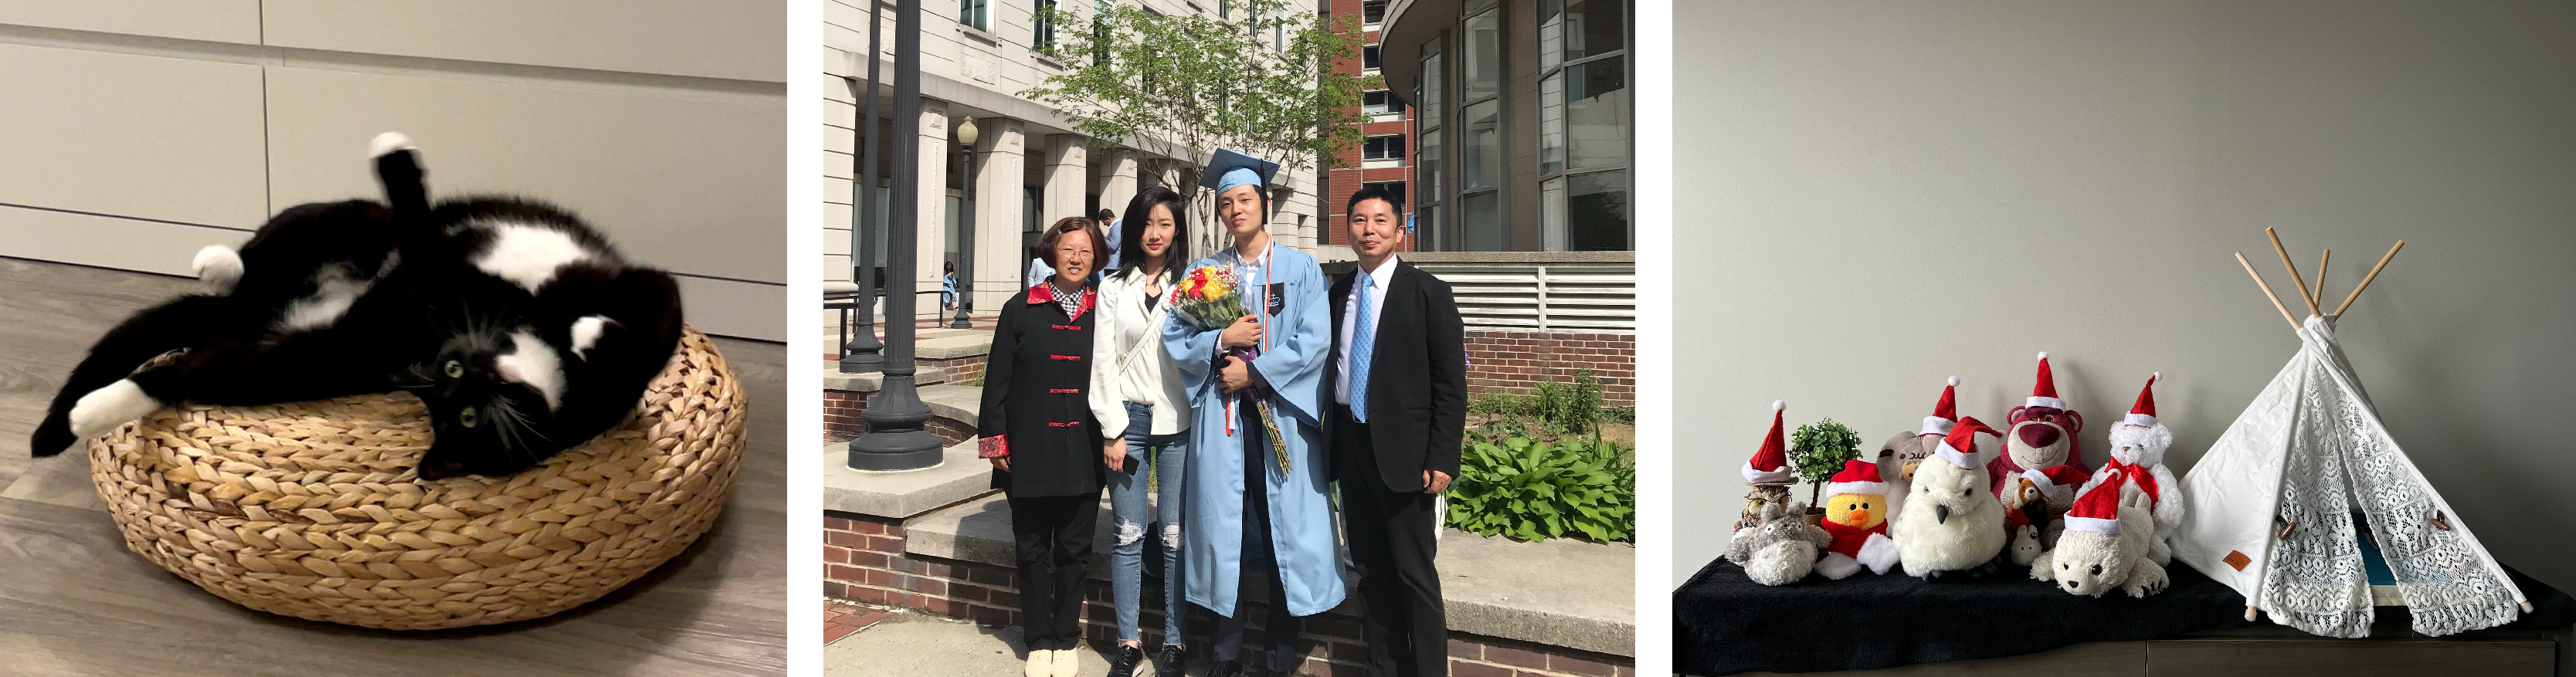
\includegraphics[width=\linewidth]{assets/fam.pdf}
    \caption{The family of the author \figloc{left to right}: Lee ``LK'' Kuai (李逵), Mingxia Wang (王明霞), Yuchen ``Reese'' Sun (孙雨晨), Dinghua Ni (倪定华), and stuffed animals (pictured Qiuqiu, Touying Mao, Lili, Sam Sun, Mengmeng, Dede, Meixiong Cao, Maotou Xiao, Keli Qiao, and Nini Ni, all in Christmas hats).}
    \label{fig:fam}
\end{figure}

Per convention, the most important humans and non-humans in my personal life are reserved for the last part of this. Non-humans first: Lee ``LK'' Kuai (李逵) is our cat, and he supported both my girlfriend and I in the final stretch of my Ph.D. and the first year of my girlfriend's career. Call me weird, but I treat stuff animals with respect and love, and I appreciate my own family of them. See \cref{fig:fam}, \figloc{left} and \figloc{right}, for cute photos of them.

Yuchen ``Reese'' Sun (孙雨晨) is my girlfriend and best friend in the last decade. We met at Dickinson College and spent the years between 2016 and 2024 in a long-distance relationship. I'm grateful for our relationship and feel extremely fortunate to have her in my life. Despite the distance, she's always been there for me. In many ways, I've been a pretty terrible partner, but she puts up with me and made me a better man. Although I dropped loads of friends' names in the preceding pages, she's my best, and depending on the definition of friendship, only friend. I'm excited to finally reunite with you after this Ph.D. ordeal, and look forward to our life together in the very near, and far, future.

I do believe I'm the luckiest son in the world because I have the best parents: Mingxia Wang (王明霞) and Dinghua Ni (倪定华). They gave their all to raise me, and, crucially, gave me the agency to make all decisions in life. My parents, like many Chinese parents, value education greatly, but, unlike most, never forced me to excel in school. My childhood and teenage years were filled with joy because of this important decision. In addition, I never took my education for granted: these are my decision, and my parents sacrificed everything to support my decisions. I cannot express my gratitude in words. My parents and I spent the majority of my Ph.D. apart since the SARS-CoV-2 pandemic in early 2020, and I miss them dearly. Out of my own decision, I always finish my academic degrees for them. I'm sure this Ph.D. will can make you both proud, and you deserve to be proud not for my achievements, but for being the greatest parents. See you in my next, and final, graduation after this.

